\chapter{Integration of Transcriptomic with Proteomic data}\label{ch:Integration}
After assessing the similarity of the human gene expression profiles
across various tissues
at transcriptomic level (with \Rnaseq\ studies in \Cref{ch:Transcriptomics})
and proteomic level (with \emph{bottom-up} \ms\ studies in \Cref{ch:proteomics}),
my next step is to examine how these gene expression profiles
compare between these two different biological layers.

One major aim of this study is to asses
how the correlations between the transcriptome and proteome
described in the literature (and mostly measured in cells)
hold at tissue level.
Moreover, good correlations may potentially lead to
the development of new strategies.
These may use the expression levels of \mRNA\ as proxies
to estimate protein expression,
which is generally difficult to measure directly (see \Cref{sec:exploreProtMS}).

I have performed the integration and all the analyses presented in this chapter
under the supervision of \alvis\ and \jyoti.
A manuscript describing this work
and the new method of protein quantification, presented in \Cref{sec:NewQuantProt},
is being prepared.

A few closely related studies~\mycite{SciRep2016,Franks2017-bp} have
been published while I was working on
the integration of the non-diseased human transcriptome and proteome.
As their analyses rely on the same data sets (\ie\ \uhlen, \gtex, \pandey\ data)
that I include in my work,
I describe and discuss together my results and theirs
whenever relevant.

\derivativeWork{}
\begin{itemize}[topsep=0pt,nosep]
    \item (poster) CSHL  Biology of Genomes 2015 --- A feasibility study:
        Integration of independent human \Rnaseq\ and proteomic datasets
\end{itemize}

\clearpage\

\vspace{-1cm}

One on-going debate in the literature is
whether good correlations of expression levels should prevail or not
between matching \mRNAs\ and proteins \mycite{Uhlen:2016}.
The implicit assumption of a proportional relationship is persisting
because of the many remaining technological limitations \mycite{Vogel2012-sq},
whereas to date, the existence of a given \mRNA\ transcript or its concentration
are usually insufficient to ensure detection of the protein in a sample.

On the one hand,
\citet{Ramakrishnan2009-lv} report that
\mRNAs\ abundance are roughly sufficient to predict
the protein presence or absence from a sample and
\citet{Vogel2010-ux} that
\mRNA\ level estimations and sequence features are enough to predict
two-thirds of the human protein abundance variation.

On the other hand,
there is a lack of high correlations
between the transcriptome and proteome
(for any organism) observation in the literature.
Previous investigations found low or no correlation
between the observed expression profiles of the \mRNAs\ and
proteins~\mycite{Anderson1997-le,Chen2002-ob,Tian2004-hh,Pascal2008-gh,%
Gry2009-zv,Lundberg2010-gk}.
This observation lack is unrestricted to human \mycite{Ghazalpour2011-nb} or
even mammals~\mycite{Gygi1999-fl,Maier2009-pb,Maier2011-tz,Yeung2011-sl,%
Palmblad2013-ji,Freiberg2016-fu}.

Additionally,
Schwanhäusser et al.~\mycite{schwanhausserglobal:2011,Schwanhausser2013-et}
present rather moderate correlations ($r^2≤0.41,\ie~r<0.64$)
for their encompassing experiment
and highlight that \mRNAs\ levels explain only about 40\% of protein variations
they have observed.

Other studies tried to explore the \mRNAs\ and proteins relationship in answer
to stimuli.
\citet{Marguerat2012-sn} report for yeast that
steady-state cells present an equivalent level of correlation ($r^2=0.36,
\ie~r=0.6$) to the previous studies,
while proliferating cells present higher correlations ($r^2=0.55, \ie~r=0.74$).
\citet{Jovanovic2015-wv} identify \mRNA\ fold changes
as the most prominent contributor to the relative changes in protein expression
for 89\% of the mouse immune genes of their study,
before concluding that relative changes in \mRNAs\ levels can explain
\emph{relative} changes in protein levels,
while post-transcriptional regulations (including degradation rates)
better explain the \emph{absolute} amount of proteins.

While many other regulations processes may occur,
post-transcriptional modifications and technical noise
are (still) perceived as the probable primary sources
of \mRNA/protein concentration discrepancies~\mycite{Vogel2012-sq,Plotkin2010-ug}.
Although
the joint study of transcriptome and proteome has already helped to highlight
links between genotype and phenotype~\mycite{Vogel2012-sq},
the previous mitigated results probably explain the focus shift of
many subsequent studies.
Previous efforts were about linking the actual expression levels.
More recent studies primarily compare qualitative attributes
of given proteins and related \mRNAs,
such as their presence or absence in a specific condition
or tissue~\mycite{Santos2015-rj,Freiberg2016-fu,Uhlen2015}
or their differential expression profiles across the same set of conditions
to detect any discrepancy~\mycite{Varemo2015-uk}.

All (or almost all) aforementioned studies have all turned to cells
for their joint analyses of transcriptome and proteome.
The analyses and integration I present in this chapter are,
on the contrary, based on tissue studies.

\vspace{-2mm}
\section{Data~and~principal~analytical~approaches}\label{sec:IntegrationData}
\vspace{-4mm}
Since 2014 and the human proteome drafts \mycite{PandeyData,KusterData},
this is the first time with such
an unparalleled availability of large-scale tissue studies
both at the transcriptomic and proteomic layers to explore and integrate together
(see \Cref{ch:datasets}).
While these data are independent
(collected from various individuals, prepared,
and characterised by different laboratories),
their combined study may help
to shed light on the relationship
between the transcriptome and proteome at the tissue level.
Using different sources for the transcriptome and proteome
increases the overall technical noise,
but it may also help to highlight relevant biological signals (as
they need to be stronger than the noise and batch effects to be captured).

In \Cref{ch:Transcriptomics}, I show that
the transcriptome \Rnaseq\ datasets present high correlations
(median value for Pearson: $r_{\setOneMath}=0.75$; $r_{\setTwoMath}=0.85$ ---
Spearman: $\rho_{\setOneMath}=0.88$; $\rho_{\setTwoMath}=0.93$).
For this chapter analyses,
I only consider the datasets with the highest similarity
(highest correlations) and
that incidentally comprise the greatest number of tissues
and are the two most recent studies,
\ie\ \dataset{Uhlén \etal}~\mycite{Uhlen2015}
and \dataset{Gtex}~\mycite{GTExTranscript} data.\\
\vspace{-\baselineskip}

Since I am reusing published data,
the initial experimental designs are suboptimal for my study.
Using both \uhlen\ and \gtex\ data
allows filtering out \mRNAs\ with high variability.
Whether this variability is technical or biological is irrelevant;
in both cases,
interpreting the relationship
between a highly variable \mRNAs\ and its protein from another dataset
remains hard to interpret.
Besides, the comparison of the two transcriptomic data may give a reference,
\ie\ an ideal case scenario, for the proteomic/transcriptomic one.

On the other hand,
the technical variability prevails over
the biological signal of same-tissue samples
for the available high-throughput proteomics,
as shown in \Cref{subsec:protTechVarHigh}.
To avoid an overly restricted protein set for the following analyses,
I only include one proteomic study: \pandey\ et al.~\mycite{PandeyData}.
All its samples have been run through the same \ms\ platform and
with the same protocol.
Besides, it presents more homogeneous protein distributions
(see \Cref{fig:distribProt} and \Cref{fig:pandeyDistribQ1Q2}) and
quantifies more proteins per tissues (\Cref{fig:distribProtUniq3D})
than the two other datasets.
As one of the main current limitations of bottom-up \ms\ proteomic studies
is the possible lack of detection of proteins for various reasons
(see \Cref{subsec:simpleProt}),
it suggests that
the \pandey\ data has a higher quality than the two other datasets.

%Many strategies are recommended to increase the depth of the coverage
%(\eg\ \mycite{Zhang2014,Eriksson2007-si,Koziol2013-si}).
%Put together these facts suggest that
%the \pandey\ data has a higher quality than the two other datasets.
\vspace{-0.5mm}
As the literature reports that
the proteome is more conserved than the transcriptome
(across individuals and species)~\mycite{Laurent2010-rg,Liu2016-re},
this data collection ought to provide a crude estimate
on the extent of observations that hold from cell to tissue level.

This chapter integration and analyses are based on the common set of tissues
and matching pairs of \mRNA/proteins.

\vspace{-2.5mm}
\subsection{Overlapping set of tissues for the three datasets}

\begin{figure}[!htbp]
    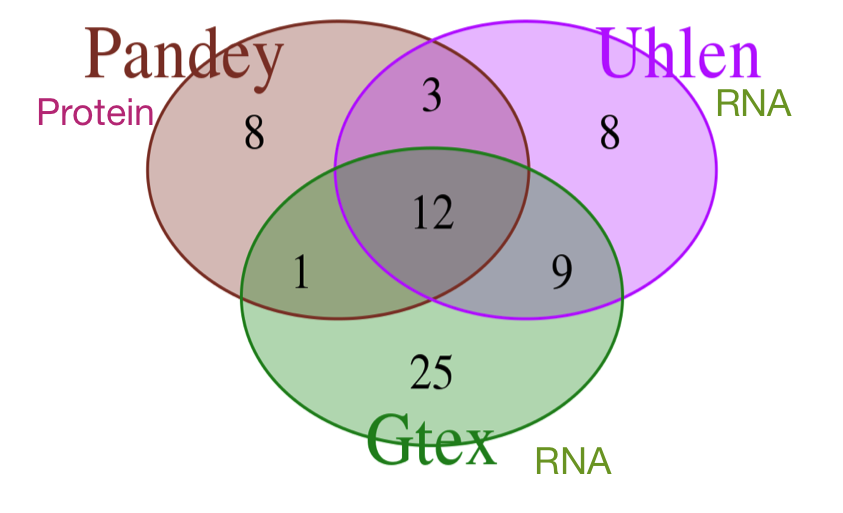
\includegraphics[scale=0.61]{integration/PandeyGtexUhlen_tissuesVenn.pdf}
    \centering
    \vspace{-5mm}
    \caption[Number of share and unique tissues between the proteomic
    dataset from Pandey \etal\ and the transcriptomic datasets (Uhlén \etal\ and
    Gtex)]{\label{fig:VennTissuePandeyGtexUhlen}\textbf{Number of share and unique
    tissues between the proteomic (Pandey \etal) and the
    transcriptomic (Uhlén \etal\ and GTEx) data.} The twelve common tissues of
    the three datasets are:
    \tissue{Adrenal gland}, \tissue{Bladder}, \tissue{Colon}, \tissue{Oesophagus},
    \tissue{Heart}, \tissue{Kidney}, \tissue{Liver}, \tissue{Lung}, \tissue{Ovary},
    \tissue{Pancreas}, \tissue{Prostate} and \tissue{Testis}. The three added
    tissue between \dataset{Uhlén \etal} and \dataset{Pandey \etal} are:
    \tissue{Gall bladder}, \tissue{Placenta} and \tissue{Rectum}. The added tissue
    between \dataset{GTEx} and \dataset{Pandey \etal} is the \tissue{Frontal
    cortex}.}
\end{figure}

All the analyses are including the twelve shared tissues between the three
datasets (\adrenal, \Bladder{}\footnote{May also
be referred as \tissue{Urinary Bladder}},
\hColon, \Oesophagus, \Heart,
\Kidney, \Liver, \Lung, \Ovary, \Pancreas,
\Prostate\ and \Testis).

\vspace{-1.5mm}
In a few cases, I have also extended the analyses by excluding the \gtex\ data
to include the three added tissues shared by
\pandey\ et al.\ and \uhlen\ et al.\ data (\ie\ \Gall, \Placenta\ and \Rectum).

\vspace{-2mm}
\subsection{Matching pairs of mRNAs and proteins}

\vspace{-3mm}
As formerly described in \Cref{sec:bias_sources},
to avoid unnecessary biases I only consider for the following analyses
\mRNAs\ (\ie\ \glspl{RNA} with a \emph{protein-coding} biotype --- \ens{76})
and proteins that are found in each dataset at least in one of the included tissues.

Besides, while there is only one value per protein per tissue,
both \uhlen\ \etal\ and \gtex\ data present replicates,
\ie\ there are several values per \mRNA\ per tissue
for each of the transcriptomic datasets.
Thus, I use the \enquote{virtual references},
\ie\ \treps\footnote{\glsdesc{TREP}}
that I describe in \Cref{subsec:averagedTissue},
to avoid unbalancing the analyses.

\begin{figure}[!htpb]
    \includegraphics[scale=0.65]{integration/PandeyGtexUhlen_mRNAprotQ1Venn.pdf}\centering
    \vspace{-5mm}
    \caption[Distribution of the unique and shared proteins/mRNAs for the three datasets
    across twelve tissues]{%
    \label{fig:PGU_vennQ1}\textbf{Distribution of the unique and shared proteins
    of Pandey et al.\ data and \mRNAs\ from Uhlén et al.\ and GTEx ones across
    their twelve shared tissues.}
    There are 6,357 matching gene products between the three datasets.
    Only 5 proteins have apparently no matching partners
    in the \uhlen\ \etal\ or \gtex\ data.}
\end{figure}

\Cref{fig:PGU_vennQ1} presents the proteins from the \pandey\ \etal\ data
quantified through the pipeline described in \Cref{subsec:msDataProcess}
and the \mRNAs\ of \uhlen\ \etal\ and \gtex\ data quantified by \htseq\
(see \Cref{subsubsec:RnaseqDataProc}).
Almost all proteins are matching to a \mRNA{}.
\Cref{fig:PU_vennQ1} is the same analysis and result
with the three added tissues shared solely by \pandey\ \etal\ et \uhlen\ \etal\ data
and without the \gtex\ data.

\begin{figure}[!htpb]
    \includegraphics[scale=0.65]{integration/PandeyUhlen_mRNAprotQ1Venn.pdf}\centering
    \vspace{-3.5mm}
    \caption[Distribution of the unique and shared proteins/mRNAs for Pandey et al.\
    and Uhlén et al.\ across fifteen tissues.]{%
    \label{fig:PU_vennQ1}\textbf{Distribution of the unique and shared proteins/mRNAs
    for Pandey et al.\ and Uhlén et al.\ across their fifteen shared tissues.}
    The number of matching pairs (6,428) and proteins that lack a counterpart in
    the transcriptomic data (8) are similar regardless on how many different
    transcriptomic data is included (see \Cref{fig:PGU_vennQ1}).}
\end{figure}

As shown in \Cref{fig:PGU_vennQ1,fig:PU_vennQ1},
only about 32\% of the quantified \mRNAs\ in the \uhlen\ \etal\ and \gtex\ data
have a corresponding proteins in the \pandey\ \etal\ data.
The protein quantification (provided by \james) follows
a state-of-the-art protocol and very stringent parameters.
Accurate protein quantification is paramount for reliable proteome exploration.
However, since my aim is to integrate proteomic data with transcriptomics,
more flexible protein identification and quantification are possible.

The new quantification that I devised for the purpose of this chapter analyses
was implemented by \james.
As described in \Cref{sec:NewQuantProt},
it is based on an \Rnaseq\ quantification approach and
takes advantage of the \emph{degenerate} peptides
to allow the quantification of proteins
even if they only have two unique peptides.

\begin{figure}[!ht]
    \includegraphics[scale=0.62]{integration/PandeyGtexUhlen_mRNAprotQ3Venn.pdf}\centering
    \vspace{-4mm}
    \caption[Distribution of the unique and shared proteins/mRNAs
    across the three datasets and twelve tissues
    (with the new protein quantification method)]{\label{fig:PGU_venQ3}%
    \textbf{Distribution of the unique and shared proteins/mRNAs
    across the Pandey et al.\ (processed with the new quantification method),
    Uhlén et al.\ and GTEx data across their twelve shared tissues}.
    }
\end{figure}

\begin{figure}[!ht]
    \includegraphics[scale=0.62]{integration/PandeyUhlen_mRNAprotQ3Venn.pdf}\centering
    \vspace{-4mm}
    \caption[Distribution of the unique and shared proteins/mRNAs for the
    Pandey et al.\ (processed with the new quantification method) and Uhlén et al.\ data
    across the fifteen tissues.
    ]{\label{fig:PU_vennQ3}\textbf{Distribution of the
    unique and shared proteins/mRNAs} for
    the Pandey et al.\ (processed with the new quantification method)
    and Uhlén et al.\ data across the fifteen tissues.}
\end{figure}

\Cref{fig:PGU_venQ3,fig:PU_vennQ3} are
the counterparts of \Cref{fig:PGU_vennQ1,fig:PU_vennQ1}.
With the new quantification method for the \pandey\ \etal\ data,
about 62\% of the \mRNAs\ quantified in the \uhlen\ \etal\ and \gtex\ data
are matched to a protein.

After comparing the respective lists of quantified proteins and \mRNAs,
I have excluded the unmatched proteins and \mRNAs\ from the following analyses
which only include the matching \emph{defined}\footnote{See \Cref{sec:ExpressedOrNot}.}
proteins and \mRNAs\ triplets (or pairs
depending on the inclusion or not of the \gtex\ data).
The lists of proteins lacking a matching \mRNAs\ in \ens{76} is provided
in \Cref{tab:protNoTrans}.

Whether or not it reflects the biological reality,
current technology detects more individual \mRNAs\ than proteins
as confirmed by \Cref{fig:UniqExprPC1,fig:distribProtUniq3D}.
Thus, it may be primarily surprising that
a few proteins lack a match in the transcriptome data.
There are several possible explanations.

Artefacts or technical issues are the most likely.
The annotation of the matching \RNA\ is missing
or is defined with another biotype than \emph{protein-coding}.
Peptides and \mRNA\ reads may be assigned to different gene IDs.
The \mRNAs\ are present in the sample,
but the library preparation has missed their capture
(see \Cref{subsec:libPrep}).
The presence of proteins in the sample is a false positive
or the result of a contamination.

However, an underlying biological phenomenon is also a possibility.
The \mRNAs\ have a very low turnover while the proteins are very stable;
The proteins are expressed elsewhere before being imported in the studied tissue
(\eg\ hormones or cytokines).

Lastly, as the transcriptomic and proteomic samples are independently sourced,
the protein may be specific to an individual or a population.
This last hypothesis is the most unlikely as there are several biological replicates
on the transcriptomic side.
Of course, a mixture of the previous causes is highly probable.

Finally, I remove from further analyses
all the proteins and \mRNAs\ from the mitochondrial genome
(see \Cref{subsec:mito}).

\vspace{-3mm}
\subsection{Tissue-centric and gene-centric approaches}
\vspace{-3mm}
\begin{figure}[!htb]
    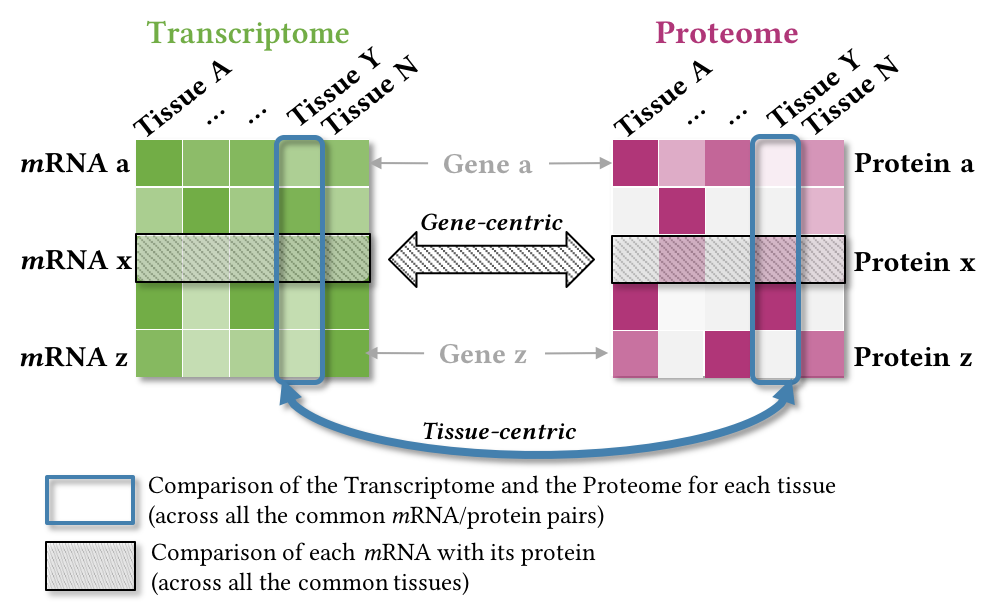
\includegraphics[scale=0.85]{integration/VisualExplaination-Lin.png}\centering
    \vspace{-3mm}
    \caption[Summary of the expression comparison approaches between
    the transcriptome and proteome]{\label{fig:visualexp}\textbf{Approaches
    summary of the expression comparison between the transcriptome and proteome.}
    \emph{Tissue-centric} analyses focus on
    how the transcriptome and proteome relate to each other within the same tissue.
    \emph{Gene-centric} analyses study for each gene how its \mRNA\ expression
    levels across all (or a subset of) the tissues may relate to
    the quantified expression levels of its corresponding protein.
    }
\end{figure}

\Cref{fig:visualexp} summarises the two analytical approaches I use
to compare transcriptomic and proteomic data.
In fact,
\citet{Liu2016-re} emphasise how important it is to clearly define
the approach when reporting results to avoid many confusions.
The \emph{tissue-centric} approach compares for each tissue
the global expression of its transcriptomic landscape to its proteomic one.
In contrast,
the \emph{gene-centric} approach compares for each gene
the expression levels of its \mRNA\ to its protein ones across all the tissues.

Note that while I use both tissue-centric and gene-centric approaches
in \Cref{ch:Transcriptomics,ch:proteomics},
explicit indications are unnecessary for their analyses.
\mRNAs\ profiles are similar enough and the proteomic studies are so disparate
that even if a confusion happens,
global understanding remains unaffected.


\section{Fair correlations between independently sourced proteomics~%
and~transcriptomics~of~human~tissues~}\label{subsec:IntegrationGoodCorrProtTrans}

As first tissue-centric analysis,
I have calculated the correlation between
the proteome and the transcriptome expressions for each tissue,
\ie\ for each tissue,
I assess the relationship between its protein expression values
to its corresponding \mRNAs.

Since the expression profile of the proteomic \treps\ and the transcriptomic ones
are similar in shape at logarithmic scale
and roughly correspond to a Gauss distribution
(see \Cref{fig:distribTrans,fig:pandeyDistribQ1Q2}),
I use both the Spearman and Pearson correlation methods
(see \Cref{sec:CorrMore}) to compare them once scaled ($\log_2{x+1}$).

\vspace{-3mm}
\begin{figure}[!htbp]
    \includegraphics[scale=0.8]{integration/DFtestlog2.pdf}\centering
    \vspace{-4mm}
    \caption[Distribution of Pearson and Spearman correlation coefficients
    for same-tissue proteomic and transcriptomic pairs
    versus random tissue pairs]{\label{fig:TestSig}\textbf{Distribution of
    Pearson and Spearman correlation coefficients
    for same-tissue proteomic and transcriptomic pairs versus random tissue
    pairs ($\log_2$-scale data).} Depending on the protein quantification method,
    there are two types of distribution ranges for the Pearson correlations.
    Top3 quantification method provides lower correlation ($\text{mean} \~{} 0.11$).
    The \PPKM\ method (\Cref{sec:NewQuantProt}) produces higher correlations
    ($\text{mean} \~{} 0.5$).
    All the Spearman correlation ranges between same-tissue proteomic and
    transcriptomic \treps\ are quite similar,
    regardless of the method quantifying the proteins.
    The Spearman correlation median is above $0.52$.
    With the Top3 quantification (\ie\ pink countered boxes --- Top3 x HTSeq),
    two outliers are noticeable and they are common to the three comparisons,
    Pandey x Uhlén (12 tissues and 15 tissues) and Pandey x GTEx (12 tissues):
    the lowest Spearman correlation is \Oesophagus\ ($\rho=0.39$)
    and the highest \liver\ ($\rho=0.62$).
    Both for the Pearson and Spearman correlations,
    even when the correlations are very low,
    same-tissue pairs have always higher correlations than
    different (random) tissues pairs
    (all p-values <0.05 (Welch t-test) --- see \Cref{tab:pvalueCorrSP}).
    Thus, even the lowest same-tissue correlations are significative.
    The green boxplots, comparing the two transcriptomic datasets,
    are only represented for reference purposes.}
\end{figure}

The Spearman correlation
between these independent transcriptomic and proteomic \treps\
is equivalent to the literature description for
same-study-sampled transcriptomics and proteomics (for cells).
This is also true for the unscaled data (see \Cref{tab:pvalueCorrSP,fig:TestSigUnlog}).
As shown in \Cref{fig:TestSig},
the median Spearman correlation coefficients are above $0.5$
for matched proteomic and transcriptomic \treps\
(also referred as \emph{same tissue pairs}),
regardless of the protein quantification method
(Top3~\mycite{Silva-Top3} or \PPKM{} ---~\vref{eq:PPKM}).
For the \PPKM\ quantification %(\Cref{sec:NewQuantProt})
the Pearson correlation is closer
to the literature than for the Top3 quantification,
and also averages above $0.5$ $[$min:~$0.38$~(\Oesophagus)\;; max:~$0.61$~(\Liver)$]$.
Note that the Pearson correlation for the untransformed data is included in
$[$min:~$0.45$~(\Oesophagus)\;; max:~$0.67$~(\Liver)$]$.
Besides, removing the pairs where the \mRNAs\ is expressed below $1$ \FPKM\ gives
substantially identical results.

While the previous distributions of correlation
may imply rather modest relationships between
the independent proteomics and transcriptomics,
same-tissue pairs scatterplots (\eg\ \Cref{fig:ScatKid})
show tighter links than first suggested.
Besides, these scatterplots present a similar rough profile
despite the wide correlation ranges (see \Cref{fig:ScatterPlotAll}).

As tissue samples from proteomic studies can present high correlation
without being related (\Cref{ch:proteomics,fig:scat2DAdrenalPancreasKuster}),
I have tested with a Welch t-test~\mycite{Welch1947-rv,Welch1951-sj}
the significance of the correlation of the same-tissue pairs
by comparison to random tissue pairs;
regardless of the protein quantification or computational methods,
all the same-tissue pairs correlations are significant
(p-value<0.05 --- see \Cref{tab:pvalueCorrSP}).

\Cref{fig:ScatKid} illustrates the comparison
between transcriptomic and proteomic gene expression
for the \tissue{Kidney} between \uhlen\ \etal\ and
\pandey\ \etal\ quantified with the new \PPKM\ method.
Note that the \kidney{}'s correlation coefficient stands
in the middle of the correlation ranges,
regardless of the studies, protein quantification or correlation methods
involved in the comparison.
To optimise the visualisation,
I removed the pairs with an unmeasured \mRNA\ or proteins,
though I kept them for the correlation calculation.

\begin{figure}[!htbp]
    \includegraphics[scale=0.75]{integration/Kidney_scattplot_Q3.pdf}\centering
    \caption[Scatterplot of protein (Pandey et al./ --- PPKM quantification)
    and \mRNA\ (Uhlén \etal) expression for Kidney]
    {\label{fig:ScatKid}\textbf{Scatterplot of
    protein (Pandey et al./ --- PPKM quantification) and \mRNAs\ (Uhlén \etal)
    expression for Kidney.}
    Each point of this scatterplot represents a gene;
    it has the $\log_2$-transformed expression value
    of the corresponding \uhlen\ \etal\ \mRNA\ (\FPKM) on the x-axis and
    the $\log_2$-transformed expression value of
    the \pandey\ \etal\ protein (\PPKM) on the y-axis.
    Most of the \mRNA/protein pairs are distributed in an area
    that can be fitted by a linear function with a positive slope,
    which indicates a high correlation between \mRNAs\ and proteins expression
    levels.
    However, genes with lower expressed \mRNAs\ are more to dispersion,
    in particular \mRNAs\ that are expressed below $1$ \FPKM\ (\ie\ below $0$ on
    the x-axis).
    On the other side, genes with the highest expressed \mRNAs\ may present
    a saturation effect (\Cref{subsec:simpleProt})
    in the quantification of the protein expression.
    The highest expressed protein is \protein{\gls{HBB}}
    (\ie\ Hemoglobin Subunit Beta), which is also found in
    the five highest expressed proteins in all the other tissues.
    Likely, its presence is due to remaining erythrocytes in the samples.
    On the outer parts of the scatterplot,
    there are the respective distribution densities of the proteins and the \mRNAs.
    Whilst the correlation calculation includes every pair of \mRNA\ and protein
    the plot excludes any pair with a null element to optimise the visualisation.}
\end{figure}

A linear function with a positive slope can fit the bulk of the \Kidney\
genes (\ie\ points).
It translates the high correlation between the expression
of the \mRNAs\ from \uhlen\ \etal\ (x-axis)
and the proteins from \pandey\ \etal\ quantified with the \PPKM\ approach (y-axis).
However, there is a high dispersion for the lowest measured \mRNAs\ ($<1$ \FPKM)
and many of the highest ones.
Besides the mismatching sampling sources,
other possible explanations for the dispersion are
technical limitations (such as protein saturation effect, see \Cref{subsec:simpleProt}),
translational noise (see \Cref{subsubsec:exprTrans})
or a consequent half-life difference between the \mRNA\ and its protein.

Although the number of genes concerned by the dispersion is rather limited,
they are enough to impair the Pearson and Spearman correlation coefficients.
Removing the lowly expressed \mRNAs\ ($<1$ \FPKM) only marginally changes
the correlation coefficients,
\eg\ for \kidney,
when considering the \PPKM\ quantification for the proteins,
the Pearson correlation
increases from $0.56$ to $0.58$,
while the Spearman correlation is relatively unchanged
($0.51$ instead of $0.52$).
The changes are relatively similar
when considering the more conservative Top3 protein quantification.
The Pearson correlation $r=0.18$ increases to $0.21$.
The Spearman correlation remains unchanged ($\rho=0.52$).

A systematic exclusion of the dispersal-prone genes
(either the proteins with lowly expressed \mRNAs\
or the highly expressed \mRNAs\ with a more limited protein expression)
is impossible
as they are inconsistent from one tissue to another.
A case-by-case treatment will be necessarily.

Regardless of the protein quantification method or
the transcriptome source (either \uhlen\ \etal\ or \gtex\ study),
the results are sensibly similar.
Thus, I mostly present thereafter the results of the most extensive set
(both in terms of tissues and genes),
\ie\ the fifteen-tissue set between \uhlen\ \etal\ and \pandey\ \etal\
(quantified with the \PPKM\ method).
Note that the other combinations are provided
in the appendices (\Cref{ch:SupplIntegration})
or in electronic format.
There may be differences for individual genes through the different combinations
but the general trends are identical.

\vspace{-5mm}
\section{Mixed biological signal between the proteome and transcriptome
across the tissues}
\vspace{-4mm}

\begin{figure}[!hbt]
    \includegraphics[scale=0.8]{integration/orderedHeatmapQ3Pearson.pdf}\centering
    \vspace{-3mm}
    \caption[Heatmap based on the Pearson correlation between protein and mRNAs
    expression (alphabetically ordered tissue)]{\label{fig:orderedHeatmapPearson}%
    \textbf{Heatmap based on the Pearson correlation between protein and mRNAs
    expression (alphabetically ordered tissue)}}
\end{figure}

Many proteomic \treps\ correlate the highest with
their corresponding transcriptomic \trep\
(\eg\ \liver, \testis, \ovary, \pancreas)
but other preferentially correlate with other tissues first
(\eg\ \bladder, \Oesophagus, \gallbladder).
Besides, depending on the chosen correlation methods,
a few tissues (\eg\ \heart) can have
their proteome and transcriptome correlate preferentially or not.\\
\vspace{-\baselineskip}

In order to identify possible factors
that influence the association strength
between the proteome and transcriptome,
I explore several avenues in the following sections.

I first use a qualitative approach
where I study the effect of tissue composition (in proteins and \mRNAs)
on the correlations.
Then, in a more quantitative approach,
I examine more closely how the \mRNA\ expression profiles relate
to their respective protein ones.

\section{Influence of the expression breadth on the tissue mRNAs/protein correlation}

Scatterplots of protein expression from different tissue pairs present
global similar profiles and correlation ranges to same tissue pairs
(see \Cref{ch:proteomics} and \Cref{fig:scat2DAdrenalPandeyPancreasKuster}).
In this context,
genes (expressed both as a protein and \mRNA)
uniquely found in one tissue can have a significant impact on the correlation.
Thus, their proportion per tissue may explain
the mitigated correlation results.%\\
%\vspace{-\baselineskip}

The expression breadth, presented in \Cref{fig:expressionBreadth},
allows visualising the number of tissues
where each gene (\mRNA\ or protein) is expressed.
\Cref{fig:protBreadth} shows that
the distribution of the protein expression breadth is bimodal.
Either due to technical limitations or biological reasons,
proteins detected in a sole tissue form
the most numerous class and represent 20 \% of the overall number.
Proteins expressed in all tissues are the second most numerous class (about $~$ 16 \%);
the third class (12 \%) comprises the proteins expressed in two tissues.

On the other hand,
almost all \mRNAs\ are expressed in every tissue (\Cref{fig:mRNAbreadth0}).
One hypothesis is that tissues express a protein only
if its corresponding \mRNA\ exceeds a sufficient threshold.
Thus, I have also studied the effect on the expression breadth
of two added thresholds above which the \mRNAs\ have to be expressed.

The two new expression breadth profiles are more alike
to the proteomic one.
As shown in \Cref{fig:mRNAbreadth1},
the number of transcripts only found in one tissue increases
at the widespread $1$ \FPKM\ threshold,
which roughly equates to one \gls{RNA} in the cell~\mycite{Mortazavi2008,Hebenstreit:2011}.

The expression breadth profile of the \mRNAs\ expressed at or above $5$ \FPKM\
present a similar bimodal distribution (\Cref{fig:mRNAbreadth5}) to the protein one.
While arbitrary, $5$ \FPKM\ is a threshold commonly found
in the literature~\mycite{Uhlen2015,oneDominant,Chen2018-ln}.

\begin{figure}[!htb]
    \begin{subfigure}[h]{0.53\textwidth}
    \captionsetup{margin=0.6cm,justification=centering}
        \centering \includegraphics[width=\textwidth]{integration/breadthProtQ3--15.pdf}
        \caption{Protein~expression~breadth (\PPKM~quantification)}\label{fig:protBreadth}
    \end{subfigure}
    \begin{subfigure}[h]{0.53\textwidth}
    \captionsetup{margin=0.6cm,justification=centering}
        \centering \includegraphics[width=\textwidth]{integration/breadthmRNAQ3--15.pdf}
        \caption{mRNA~expression~breadth\\(> 0 \FPKM)}\label{fig:mRNAbreadth0}
    \end{subfigure}
    \vspace{2.5mm}

    \begin{subfigure}[b]{0.53\textwidth}
    \captionsetup{margin=0.6cm,justification=centering}
        \centering \includegraphics[width=\textwidth]{integration/breadthmRNAQ3--1501.pdf}
        \caption{mRNA~expression~breadth\\(≥1 \FPKM)}\label{fig:mRNAbreadth1}
    \end{subfigure}
    \begin{subfigure}[b]{0.53\textwidth}
    \captionsetup{margin=0.6cm,justification=centering}
        \centering \includegraphics[width=\textwidth]{integration/breadthmRNAQ3--1505.pdf}
        \caption{mRNA~expression~breadth\\(≥5 \FPKM)}\label{fig:mRNAbreadth5}
    \end{subfigure}
    \vspace{-5mm}
    \caption[Expression breadth of the proteins and mRNAs]{\label{fig:expressionBreadth}%
    \textbf{Expression breadth of the proteins and mRNAs.}
    Proteins have a bimodal breadth of expression.
    Many proteins are detected in one tissue only or in all tissues.
    Almost every \mRNA\ is detected in every tissue.
    Their breadth becomes bimodal when their expression threshold
    is increased to $5$ \FPKM{}.
    Note that the genes with null expression breadth are removed from the plots
    to ease the general visualisation.
    }
\end{figure}

\Cref{fig:UniqueFeatureQ3T15} shows the proteins and \mRNAs\
for which the expression breadth equates to $1$ in \Cref{fig:expressionBreadth}.
Instead of displaying the finite counts,
it displays the ratio per tissue,
\ie\ the number of unique feature (proteins or \mRNAs)
for each tissue divided by the total amount of them across all tissues.
The tissues are ordered in increasing order of their ratio in unique features.

\begin{figure}[!htb]
    \includegraphics[scale=0.78]{integration/uniqueFeatureQ3T15.pdf}\centering
    \vspace{-3mm}
    \caption[Ratio per tissue of unique proteins and mRNAs]{\label{fig:UniqueFeatureQ3T15}
    \textbf{Ratio per tissue of unique proteins and mRNAs.}
    }
\end{figure}

Every tissue presents proteins that are only detected in that specific tissue.
In contrast, unique \mRNAs\ are detected in a more limited number of tissues.
Besides, the unique proteins are more evenly distributed
between the fifteen tissues than the unique \mRNAs.

Except for \Testis\ and \Liver,
which are consistently expressing the highest number of unique features,
the other tissues lack to present any common pattern
between the available proteomic and transcriptomic data.

\Liver\ is the most correlated tissue (\Cref{fig:orderedHeatmapPearson})
and comprises the second highest number of unique features.
\Testis\ is the third best correlated tissue
despite having the highest ratio of unique proteins and \mRNAs\
(regardless of the threshold $0$ to $1$ \FPKM).
The other tissues lack to show any relationship
between their composition in unique features
and the correlation of their transcriptome and proteome.

Put together these results suggest that
the tissues correlation levels are unrelated
to their amount of unique proteins and \mRNAs{}.
The lack of relation between the proteomic and transcriptomic observations
is confirmed by a more refined analysis of the expression breadth.

\begin{figure}[!htpb]
    \includegraphics[scale=0.75]{integration/coloredSharedbreadthProtQ3--15.pdf}\centering
    \vspace{-4mm}
    \caption[Comparison of the proteins expression breadth to their
    corresponding mRNA ones]{\label{fig:SharedBreadthProtQ3}%
    \textbf{Comparison of the proteins expression breadth
    to their corresponding mRNA ones.}
    This figure, where the protein expression breadth is coloured
    according to its comparison with the \mRNA\ one,
    is based on \Cref{fig:protBreadth,fig:mRNAbreadth5}.
    About one fifth of the proteins that are detected in one tissue
    have their corresponding \mRNA\ (expressed at or above $5$ \FPKM{})
    presenting an \emph{identical} expression breadth.
    The number of proteins classified as \emph{Identical} decreases significantly
    for the other possible breadths
    except when all the tissues (\ie\ fifteen) are considered
    (then accounting for one third of the proteins).
    Proteins with a breath of expression close to their \mRNAs{}' (± $2$)
    are identified as \emph{Similar}.
    If the protein and the \mRNA\ are both detected within four to nine tissues,
    they are described as \emph{Mixed}.
    If the \mRNA\ has been detected at or above $5$ \FPKM\
    but with another breadth than \emph{Identical} or \emph{Similar},
    it is then referred as \emph{Different}.
    Finally, while many proteins are detected in one tissue (or even more)
    their corresponding \mRNAs\ is not at $5$ \FPKM\
    (\emph{Expression < $5$ \FPKM} category).
    }
\end{figure}

\Cref{fig:SharedBreadthProtQ3} shows that the expression breadth
of \mRNAs\ (expressed ≥ $5$ \FPKM\ or even smaller threshold) concurs
in very few cases to their corresponding protein one.
Thus, the \mRNAs\ expression breadth is
an ineffective predictor for the detection of a protein,
including extreme cases where the protein is unique to one tissue
or expressed in all fifteen of them.

Expression breadth analyses of the transcriptome rely on expression levels.
On the other hand, \Cref{ch:Transcriptomics} underlines that
high expression levels of \mRNAs\ are unrelated to interstudy tissue correlation
while tissue-specific (\gls{TS}) \mRNAs\ present a rather strong connection with it.
For this reason, one of the following analysis (\Cref{sec:TSprotMrna}) examines
the relationship between \gls{TS} \mRNAs\ and proteins.

However, I report beforehand another analysis.
After determining that it is impossible to classify the tissues consistently
based on their unique features as shown in \Cref{fig:expressionBreadth},
I explore whether the tissues conserve the same hierarchical clustering
when considering the proteins or \mRNAs\ that are expressed in two tissues strictly.

\begin{figure}[!htb]
    \begin{subfigure}[b]{0.53\textwidth}
    \captionsetup{margin=0.6cm,justification=centering}
        \centering \includegraphics[width=\textwidth]{integration/TissuePairsQ3T15Pandey.pdf}
        \caption{Pandey et al.\ tissues\\(PPKM quantification)}\label{fig:treePandeyQ3T15}
    \end{subfigure}%
    \begin{subfigure}[b]{0.53\textwidth}
    \captionsetup{margin=0.6cm,justification=centering}
        \centering \includegraphics[width=\textwidth]{integration/TissuePairsQ3T15UhlenCut5.pdf}
        \caption{Uhlén et al.\ tissues\\(≥5 \FPKM)}\label{fig:treeUhlenQ3T15cuth5}
    \end{subfigure}
    \vspace{-5mm}
    \caption[Tissues hierachical clustering for Pandey and Uhlén]{\label{fig:separateTree}%
    \textbf{Hierarchical clustering for the fifteen tissues of
    Pandey et al.\ and Uhlén et al.\ studies.}
    }
\end{figure}


\begin{figure}[!htb]
    \begin{subfigure}[b]{0.53\textwidth}
        \captionsetup{margin=0.6cm,justification=centering}
        \centering \includegraphics[width=\textwidth]{integration/TissuePairsQ3T15.pdf}
        \caption{Consensus}\label{fig:consensus2D15TQ3}
    \end{subfigure}%
    \begin{subfigure}[b]{0.53\textwidth}
        \captionsetup{margin=0.6cm,justification=centering}
        \centering \includegraphics[width=\textwidth]{integration/TissuePairsQ3T123DFconsensus05.pdf}
        \caption{<++>}\label{fig:consensusTree05}
    \end{subfigure}
    \vspace{-5mm}
    \caption[Tissues hierachical clustering for Pandey and Uhlén]{\label{fig:consensusTrees}%
    \textbf{Consensus of the hierachical clustering of the tissues across the different studies.}
    }
\end{figure}


\section{Tissue-specific mRNAs and proteins}\label{sec:TSprotMrna}

%%% Parler que unicité est différent de la specificité et que pour les mrnas,
%%% specificité est déterminé d'une autre manière.
As many proteins are only expressed in a unique tissue,
we can consider them as tissue-specific.

It appears that a direct comparison of the proteins that have been identified
with the identified \mRNAs\ (even with various thresholds) is not so meaningful.

Instead of focusing of the uniqueness of a gene (or in a broader way, the breadth
of expression),the main issue here is to
determine what and when a gene is \emph{specific}. In fact, I can not use
the same definition of detection like for the proteins. I then chose to focus
on the \emph{Tissue-Specific} genes.




\section{Gene centric studies}

As I exposed in~\Cref{ch:Transcriptomics}, there are some
\mRNAs\ that are lowly or even anti-correlated between the different
transcriptomic datasets.
As I can not pinpoint whether this is due to \emph{biological} or \emph{technical}
reasons, we choose to exclude the anticorrelated \mRNAs\ between \dataset{Uhlén
\etal} and \dataset{Gtex} (across the 23 common tissues) as these two datasets have
very similar protocols and have been sequenced on similar sequencers (Illumina
HiSeq 2000/2500).



\subsection{Tissue specific \textit{m}RNAs have significant overlap with tissue
specific proteins}

\begin{figure}[!htbp]
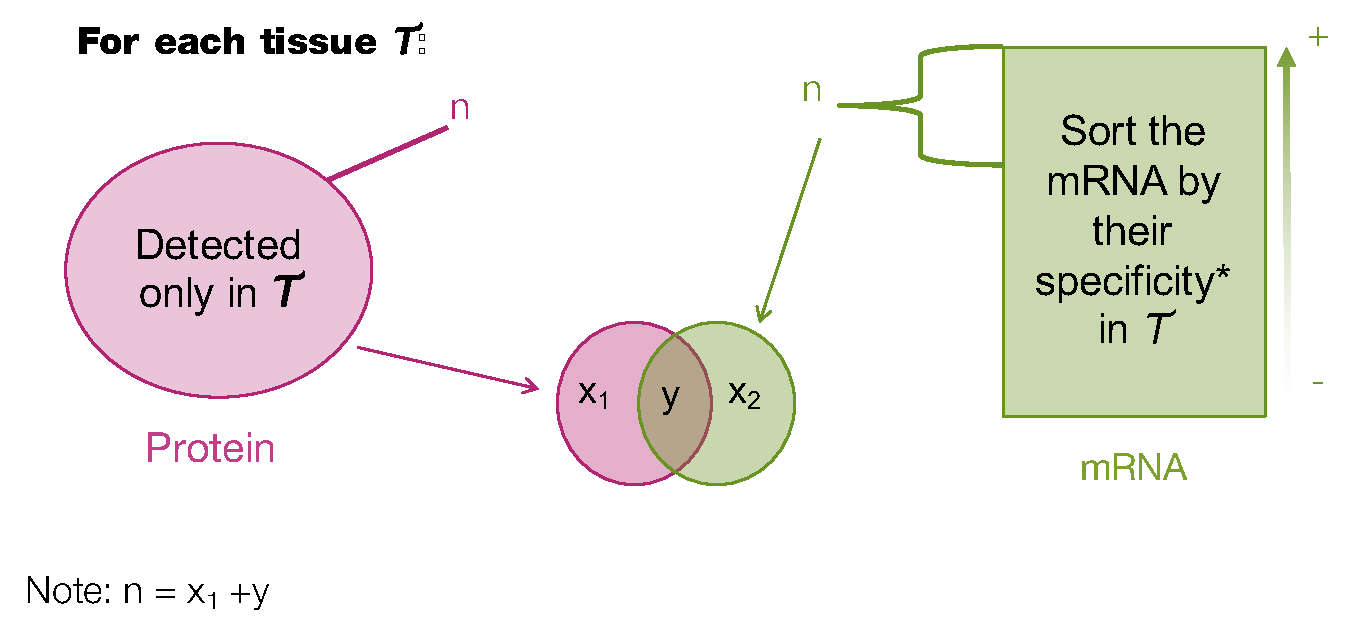
\includegraphics[scale=0.7]{integration/RankSpe}\centering
    \caption[Determination process of specific
    mRNAs]{\label{fig:RankSpe}\textbf{Determination process of specific \mRNAs.}}
\end{figure}


\begin{figure}[!htbp]
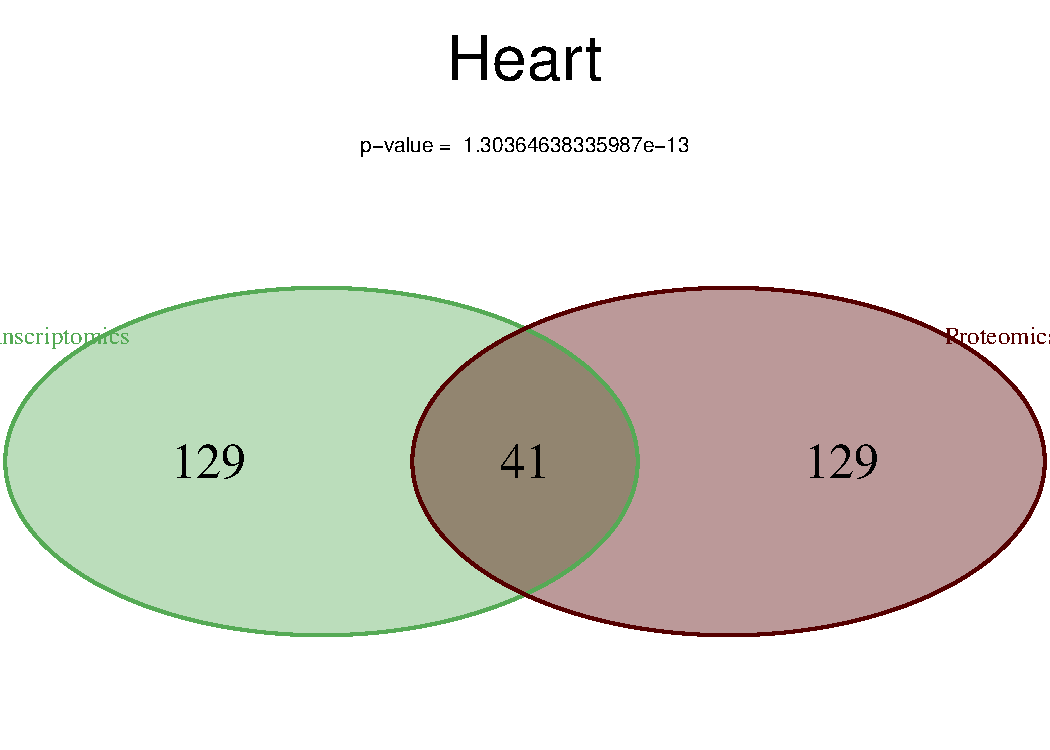
\includegraphics[scale=0.7]{integration/SpeJacquard/Heart}\centering
    \caption[Example of overlap of specific protein and specific
    mRNAs for heart]{\label{fig:ExJacquard}\textbf{Example of overlap of
    specific proteins and specific \mRNAs.}}
\end{figure}


\begin{figure}[!htbp]
\includegraphics[scale=0.4]{integration/RatioJac}\centering
    \caption[Heatmap of Jaquard indices]{\label{fig:RatioJac}\textbf{Heatmap of
    Jaquard indices.}}
\end{figure}

\begin{figure}[!htbp]
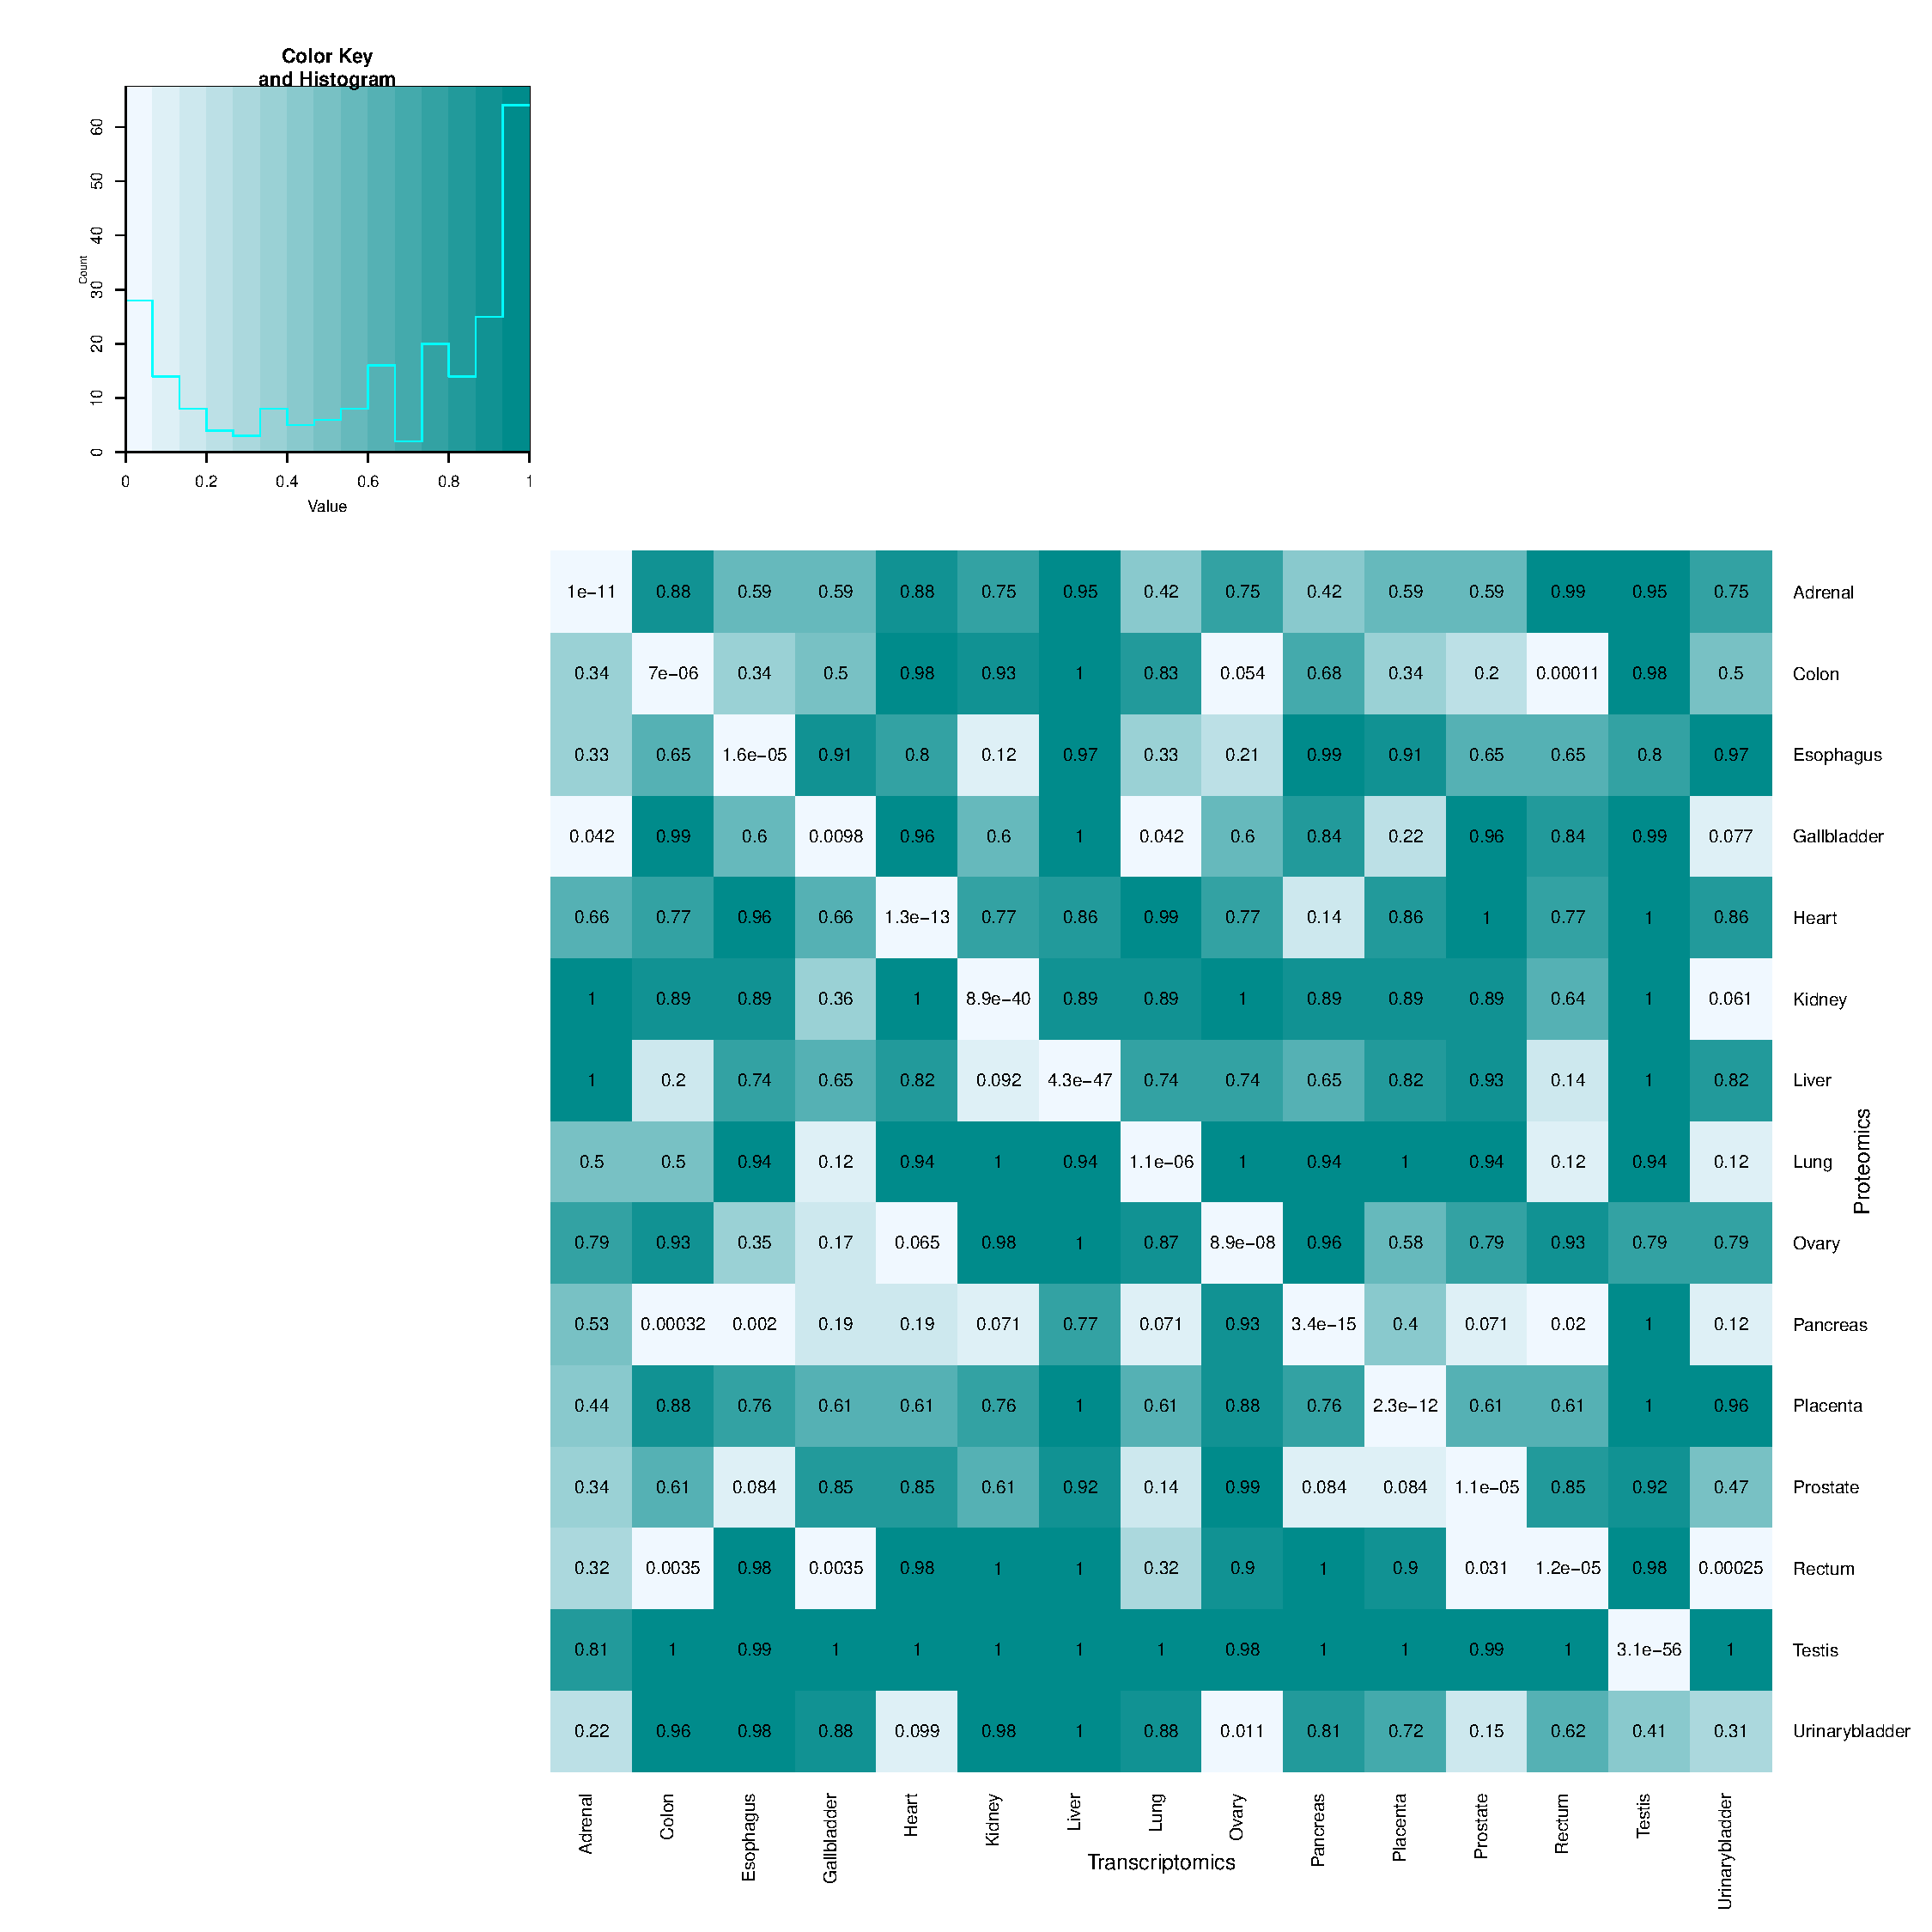
\includegraphics[scale=0.4]{integration/pJacquard}\centering
    \caption[p-values associated to the Jaquard
    indices]{\label{fig:pJacquard}\textbf{p-value associated to the Jaquard
    indices.}They have been computed with hypergeometric test.}
\end{figure}

\subsection{Expression levels of mRNAs correlate with the expressed proteins}

\begin{figure}[!htbp]
    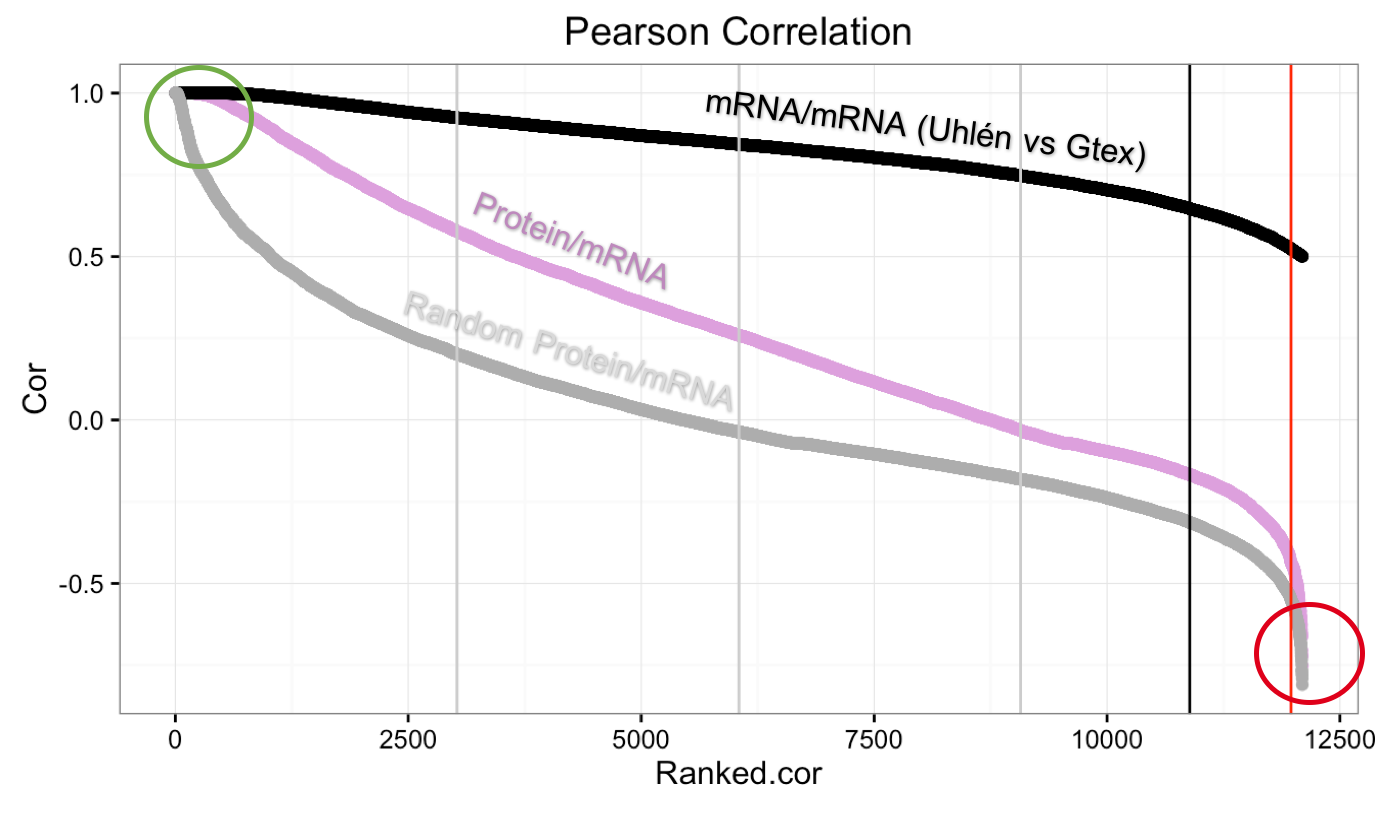
\includegraphics[scale=0.55]{integration/GeneProtCorAnno}\centering
    \caption[Pearson correlation coefficients of \mRNA/protein pairs expression
    across the common tissues in descending order]
    {\label{GeneProtCor}\textbf{Pearson correlation coefficients of \mRNA/protein
    pairs expression across the common tissues in descending order.} For each
    couple of \mRNA\ and its corresponding protein, the Pearson correlation of
    their respective expression across the same set of tissue is calculated. Then,
    all the pairs are sorted in descending order and plotted based on their
    correlation coefficient in pink. To provide context to these results,
    An \emph{ideal} case has also been calculated. The identical \mRNAs\ set of
    the current Proteome and Transcriptome comparison has been used for a
    Transcriptome (\dataset{Uhlén \etal}) and Transcriptome comparison
    (\dataset{GTEX}). We can see that even the ideal case is not a perfect
    horizontal line (which would indicate a whole and complete correlation between
    the two transcriptomic datasets).}
\end{figure}


\begin{figure}[!htbp]
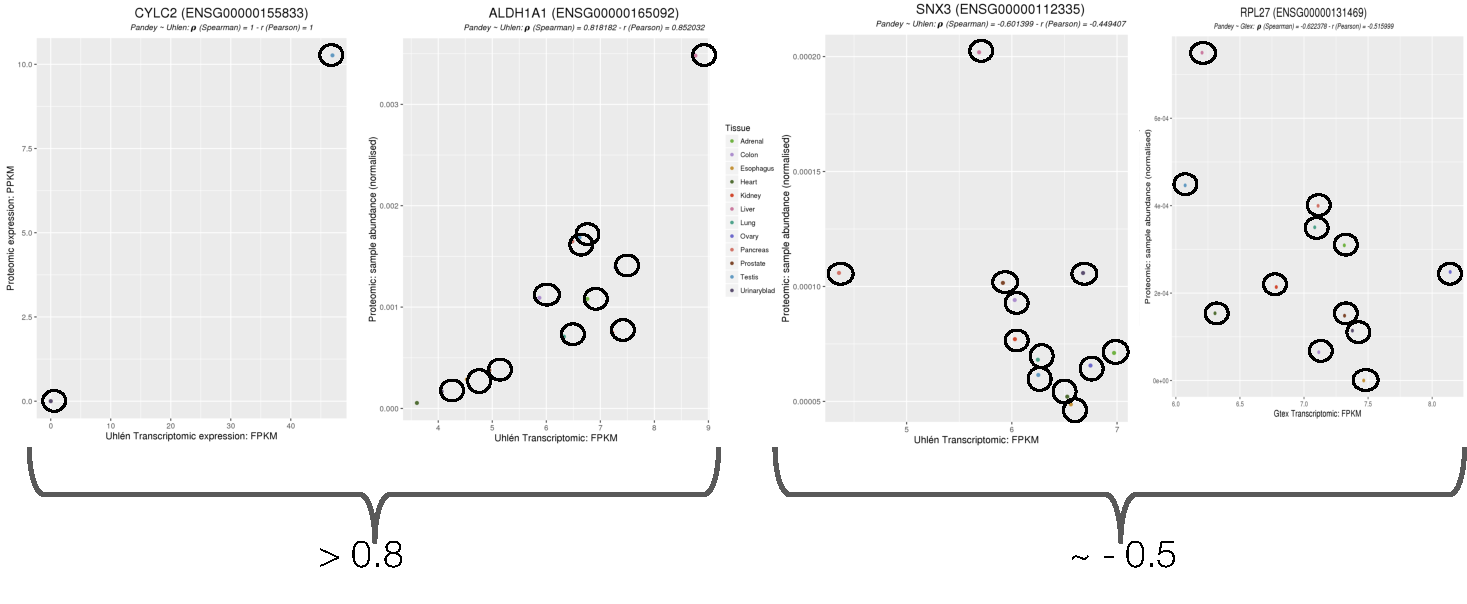
\includegraphics[scale=0.5]{integration/caseGene}\centering
    \caption[Different cases of correlation
    protein/mRNA]{\label{fig:caseGene}\textbf{Different cases of correlation
    protein/\mRNA.} The high correlated ones are enriched in pairs that are
    Tissue-specific as \mRNA\ and protein.}
\end{figure}

\subsection{Pairs composed of tissue specific proteins tend to correlate better}

\begin{figure}[!htbp]
    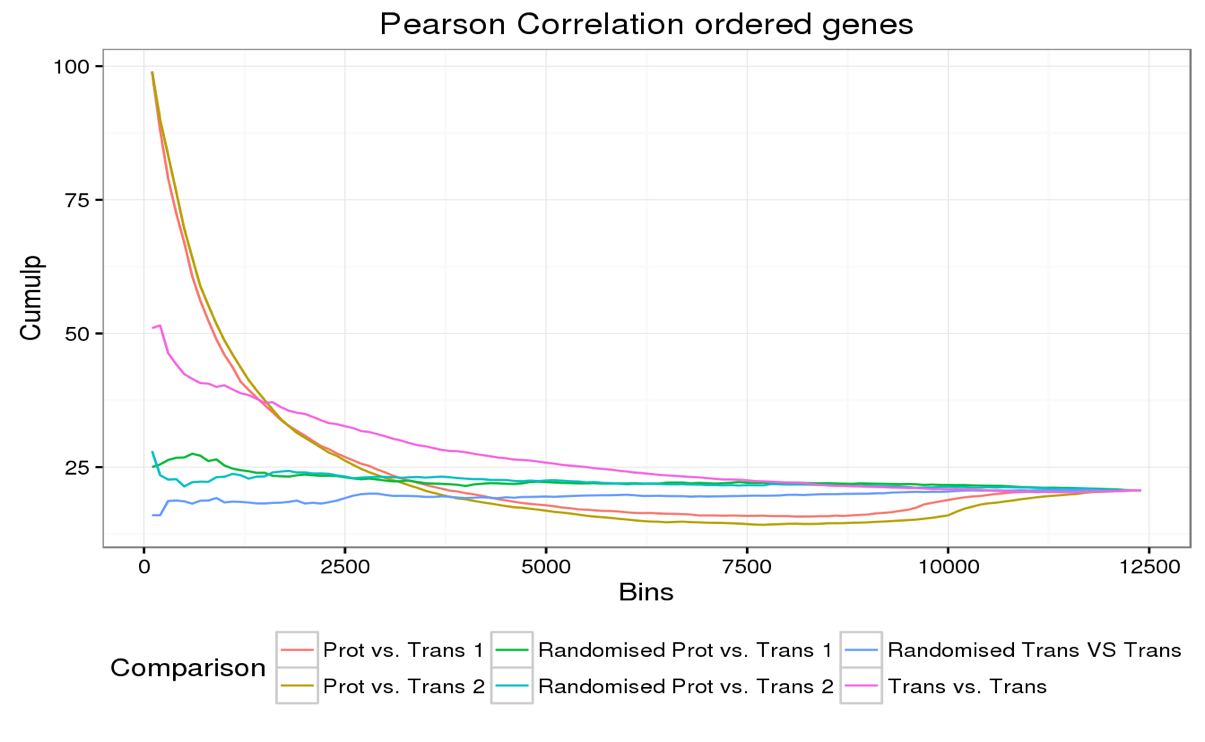
\includegraphics[scale=0.7]{integration/Spe_Cor}\centering
    \caption[Cumul ratio of the specific proteins ordered on the correlation
    of the mRNA/protein pairs across the 15
    tissues]{\label{fig:Spe_Cor}\textbf{Cumul ratio of the specific proteins
    ordered on the correlation of the mRNA/protein pairs across the 15 tissues.}}
\end{figure}


\TK{Can tissues correlations be improved by removing the lowly correlated genes? =>
it is not always the same pairs that are in the same quadrant ==> no `argument''
that would legitimate this. Ref:~\cref{fig:CorImprovable}}


\begin{figure}[!htbp]
    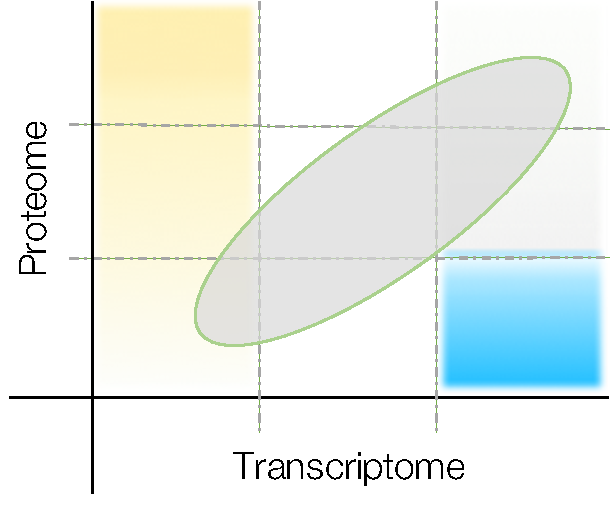
\includegraphics[scale=0.85]{integration/improvingTisseCor}\centering
    \caption[Possible biological significations of a \mRNA/protein pair based on
    its possition in the scatter plot]
    {\label{fig:CorImprovable}\textbf{Possible biological significations of a
    \mRNA/protein pair based on its position in the scatter plot.}Indeed, as all
    the scatter plots present the same shape with a saturation for the proteins
    highly expressed in each tissues and a great dispersion for the lowly
    expressed \mRNAs}
\end{figure}


\subsection{GO enrichment of the different categories}


\begin{figure}[!htbp]
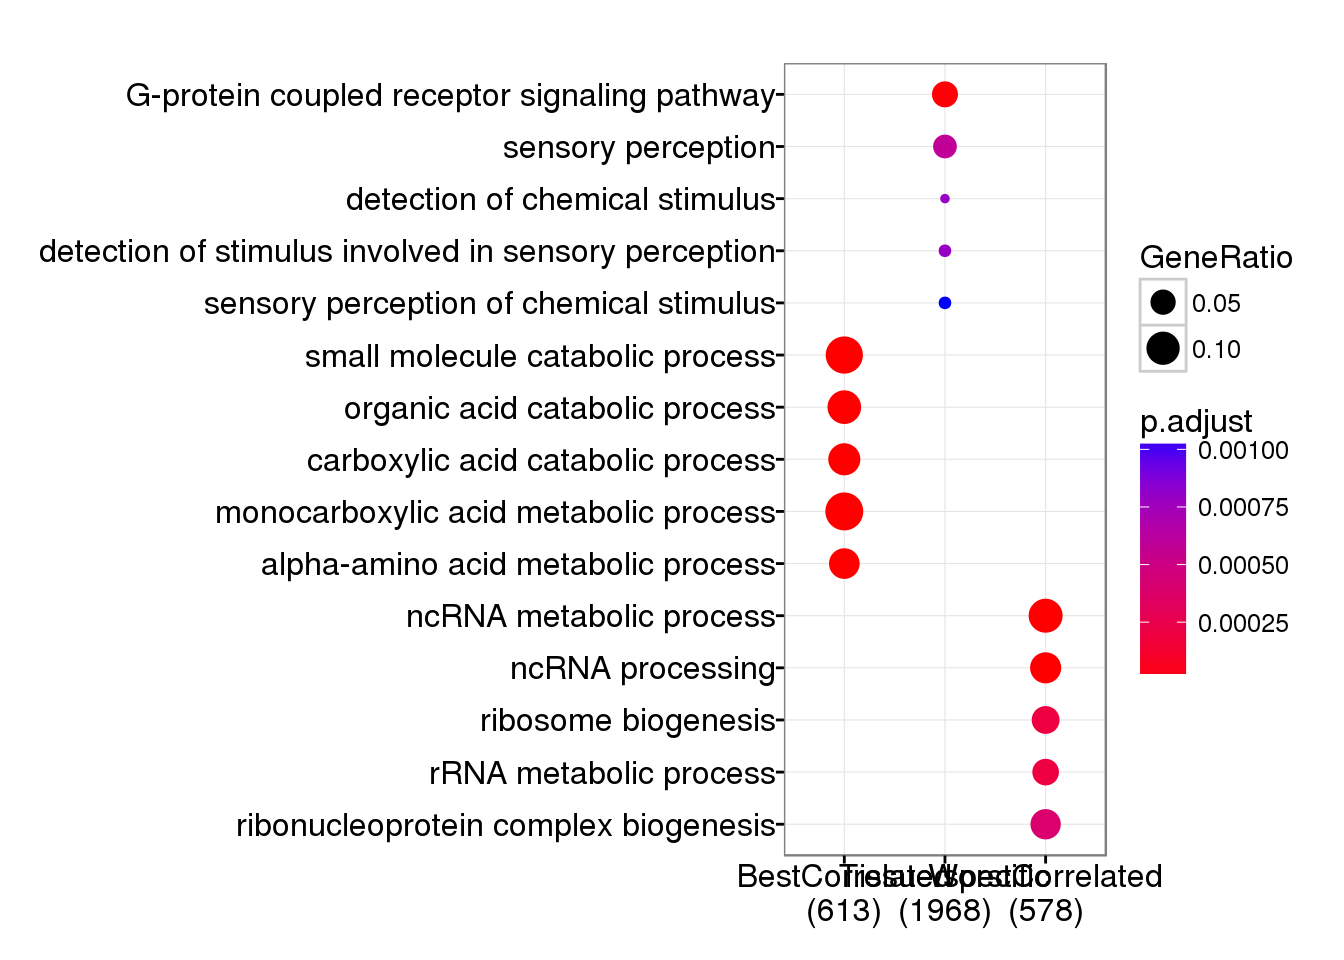
\includegraphics[scale=0.7]{integration/Go_dotplot}\centering
    \caption[GO enrichment analysis of the highest, lowest and Tissue
    specific genes]{\label{fig:Go_dotplot}\textbf{GO enrichment analysis of the
    highest, lowest and Tissue specific genes.}}
\end{figure}


\begin{figure}[!htbp]
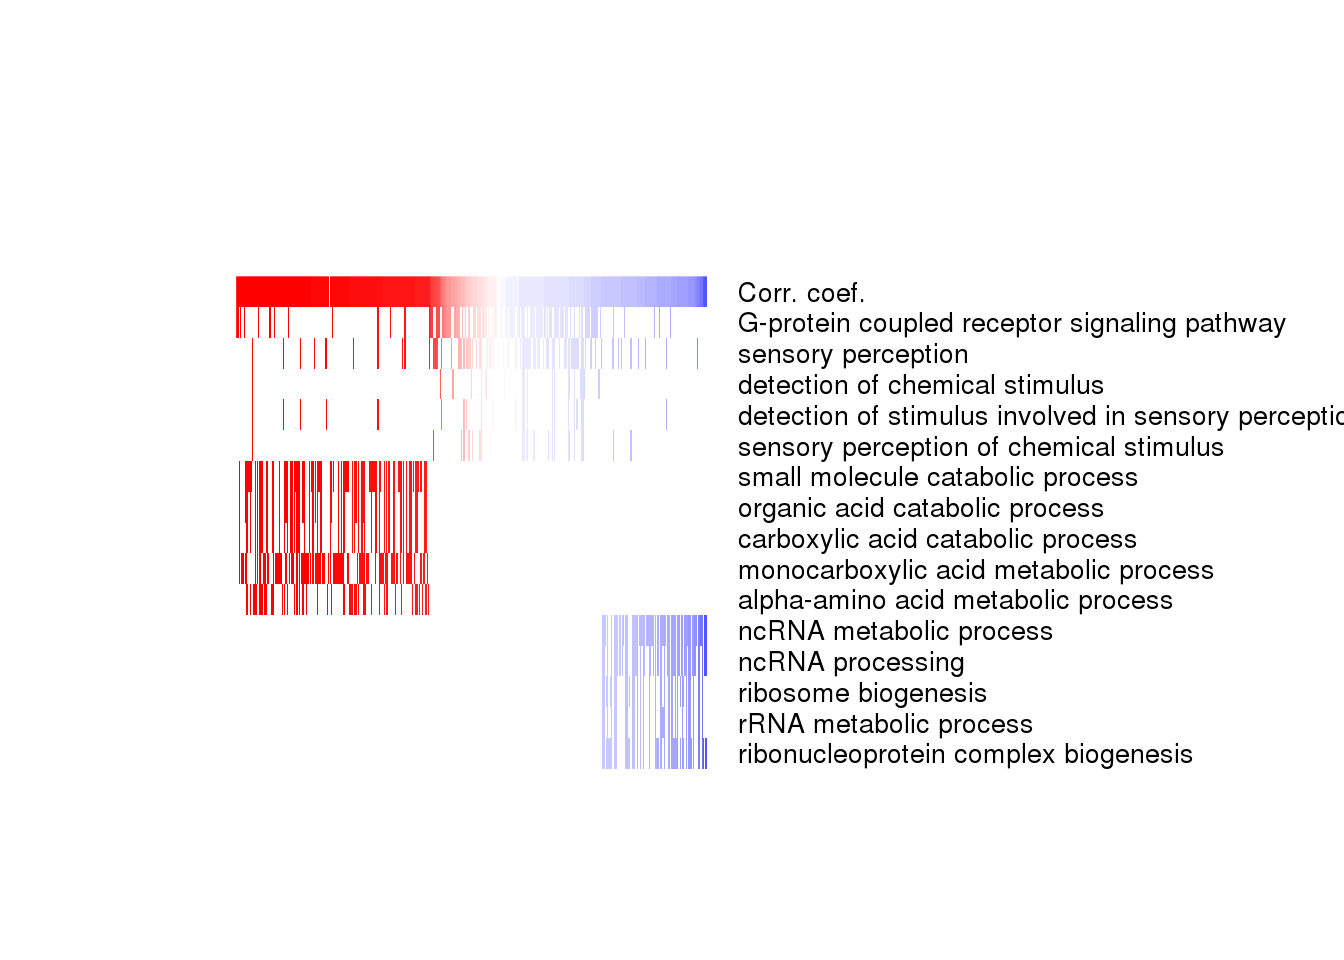
\includegraphics[scale=0.7]{integration/GO_cor_sorted}\centering
    \caption[Correlation coefficient of the pairs for the GO
    categories]{\label{fig:GO_cor_sorted}\textbf{Correlation coefficient of the
    GO categories.}}
\end{figure}


\begin{figure}[!htbp]
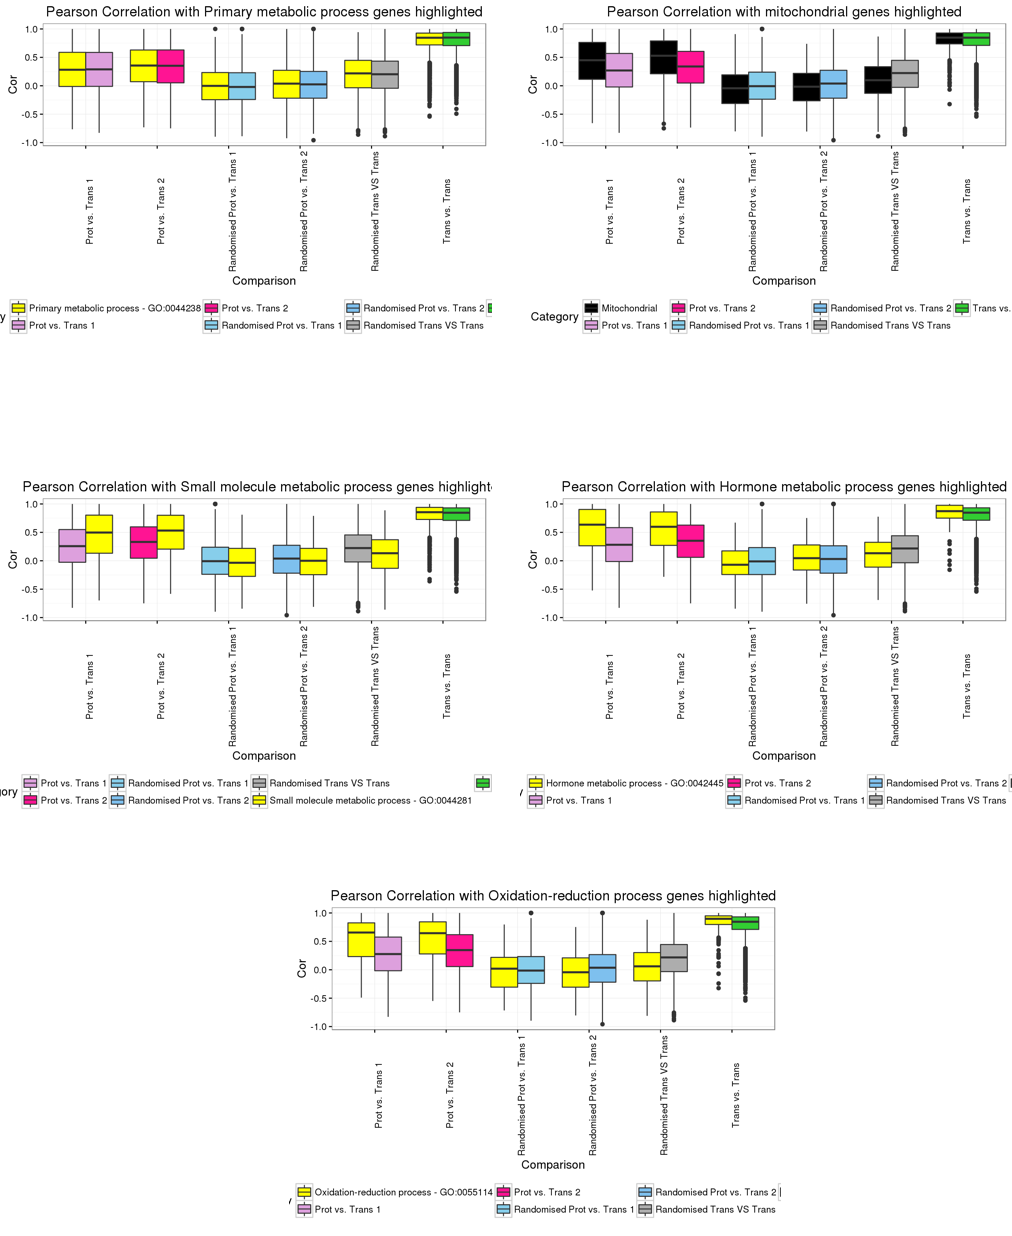
\includegraphics[scale=0.7]{integration/OtherGroups}\centering
    \caption[Examples of particular GO
    categories]{\label{fig:GO_sub_groups}\textbf{Examples of particular GO
    categories.}}
\end{figure}


%if tissue more specific (greater diversity) the proteome, true for transcript as well?
%   barplot (no cutoff) but then 1FPKM<=> 1 protein (barplot 1FPKM ? yes/no?)
%        ---> breadth of expression distribution
%          ---> barplot 5 FPKM ==> Doesn't work BUT other way to compute the
%          specificity of mRNAs--> rank then compute Indice de Jacquard!
%===> *SO* specificity can be kept between Protein and Transcript
%_but then_ quid of Expression values, do they correlate?
%        * Eh, but then show that most high correlated are the specific but not only:
%        there are also others ---> GO annotation.



\clearpage\

\section{Discussion}

Although, the range of Pearson correlation coefficients could seem average or
low, it is actually greater than the average numbers reported in the literature,
\TK{Add citation list}
particularly as the proteome and the transcriptome have completely different
biological sources.


People look at the highest and lowest expressed genes (in one condition, or very
similar conditions) for the correlation (which is supported by the scatter plot:
indeed, it seems that the greatest bulk is closely correlated) {\Large BUT} if we
want to unlock a deeper understanding of the regulation of the translation, we need
to compare multiple conditions (as all the pairs won't behave in the same fashion
depending which is the considered condition) and more importantly it's it not
really link to the ``quantile'' of expression. Indeed, the protein and the \mRNA\
might be very well correlated, but their expression levels can be somewhat disconnect.

Big plus of this analysis, not only one conditions, but multiple and can try to
avoid technical artefacts by crossing over the results. (More importantly, whatever
which would be found would be consistent with the technology and not just a fling,
\ie\ it is more robust that any of the study took by itself.)
Which is a weakness of the data (not the same people) create a force (what is found
is probably universal). (We can't say anything about the non-findings!!!)

This approach is even more important in case that you study the tissue specific
(or condition) specific pair, they globally the more correlated. (Are they actually???)

So big need of an external/outliers samples (or more) or external source.


\begin{comment}
\TK{Proteome sensé être plus conserver que le RNA : citation}
\end{comment}

%%%%%%%

%%% Check notational for the added Jaquard index analysis and some other stuff.

%%%%%%




%%%%cimetiere
%%These studies however were mostly done at cell levels.
%%While the pool of protein coding transcripts is about 60 to 70 \% similar from
%%one tissue to another, the protein pool is quite different.


% Hence, a component of the decrease in the
% correlation between the \mRNA\ and its protein is due to t The pink line,
%while more similar in essence to the random pair correlation, presents about
%500 genes/proteins pairs that    are highly correlated.


%We can also note that a broader number of tissues-specific \mRNAs\ doesn't
%necessarily imply the same at proteomic level and vice versa.
%In~\cref{fig:barPlotunique}, we can see that \tissue{Testis} and \tissue{Liver}
%are the tissues with the greatest number of tissues specific \mRNAs\ and proteins.
%The reality is more mixed for the other tissues.

%\subsection{Relative specificity of the tissues are kept from transcriptome to
%proteome level for the most extreme cases --- \ie\ proteomic diversity of a tissue
%can not be systematically deduced from transcriptomic}


%We can also note that a broader number of tissues-specific \mRNAs\ doesn't
%necessarily imply the same at proteomic level and vice versa.
%In~\cref{fig:barPlotunique}, we can see that \tissue{Testis} and \tissue{Liver}
%are the tissues with the greatest number of tissues specific \mRNAs\ and proteins.
%The reality is more mixed for the other tissues.


%As the \mRNAs\ are expressed in more tissues in general, I tried to take account for this in the following analysis I run.

Possible explanation of the anticorrelations may be due
at the number of transcript or their definition or some other
attributes that can be found in
\textbf{APRIS} (Apris transcript codant (or content?)) (suggested by Nuno).


From~\citet{Marguerat2012-sn} protein copies exceed \mRNA\ ones a lot.
And if proteins not detected for \mRNAs, proteins that are tightly regulated
(but they have different states where they can check the presence of the proteins
in the data in general).

From~\citet{Vogel2012-sq} which is citing~\citet{schwanhausserglobal:2011}
RNAs and proteins from mammalian metabolic genes tend to be very stable
and (citing~\citet{Vogel2010-ux}) have high protein-per-mRNA ratios.

\ms\ label-free absolute quantification proteomics
underestimate a large dynamic range of proteins~\mycite{TOP3isbetter}.


\citet{Edfors2016-kv} have found that cell lines derived from a tissue don't present
the same (absolute) amount of proteins than tissue samples and warned to be cautious
if cell lines are used as model for normal tissue.



